\documentclass[tikz,border=10pt]{standalone}
\usepackage[T1]{fontenc}
\usepackage[utf8]{inputenc}
\usepackage{lmodern}
\usepackage{amsmath,amssymb}
\usetikzlibrary{arrows.meta,positioning,shapes.geometric,calc}
\definecolor{jac}{HTML}{73539E}
\definecolor{ink}{HTML}{354052}
\tikzset{
 >=Stealth,
 state/.style={draw=jac,fill=jac!7,rounded corners=5pt,align=center,minimum width=26mm,minimum height=11mm,inner sep=5pt,font=\small},
 action/.style={state,fill=white},
 decision/.style={draw=jac,fill=jac!7,diamond,aspect=2.4,inner sep=1.8pt,align=center,font=\small},
 success/.style={state,draw=teal!75!black,fill=teal!7},
 failure/.style={state,draw=red!70!black,fill=red!5},
 arrow/.style={->,thick,draw=ink},
 note/.style={align=left,font=\footnotesize,text=ink}
}
\begin{document}

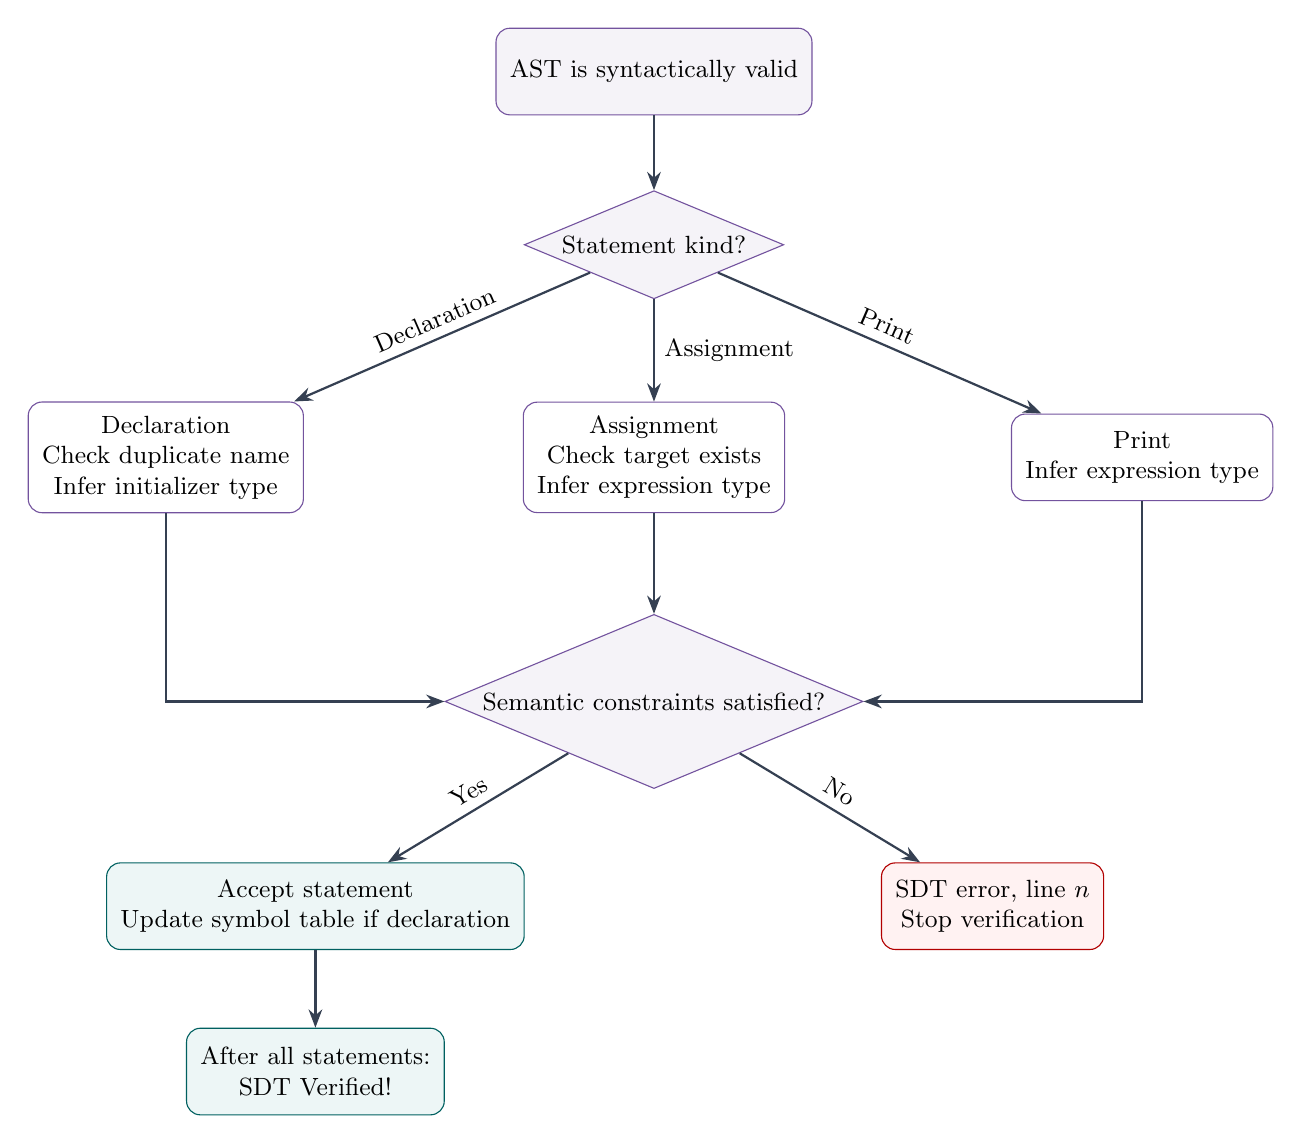
\begin{tikzpicture}[font=\small]
\node[state] (start) at (0,0) {AST is syntactically valid};
\node[decision] (kind) at (0,-2.2) {Statement kind?};
\node[action] (decl) at (-6.2,-4.9) {Declaration\\Check duplicate name\\Infer initializer type};
\node[action] (assign) at (0,-4.9) {Assignment\\Check target exists\\Infer expression type};
\node[action] (print) at (6.2,-4.9) {Print\\Infer expression type};
\node[decision] (valid) at (0,-8) {Semantic constraints satisfied?};
\node[success] (ok) at (-4.3,-10.6) {Accept statement\\Update symbol table if declaration};
\node[failure] (error) at (4.3,-10.6) {SDT error, line $n$\\Stop verification};
\node[success] (complete) at (-4.3,-12.7) {After all statements:\\SDT Verified!};
\draw[arrow] (start)--(kind);
\draw[arrow] (kind)--node[above,sloped]{Declaration}(decl);
\draw[arrow] (kind)--node[right]{Assignment}(assign);
\draw[arrow] (kind)--node[above,sloped]{Print}(print);
\draw[arrow] (decl.south) |- (valid.west);
\draw[arrow] (assign)--(valid);
\draw[arrow] (print.south) |- (valid.east);
\draw[arrow] (valid)--node[above,sloped]{Yes}(ok);
\draw[arrow] (valid)--node[above,sloped]{No}(error);
\draw[arrow] (ok)--(complete);
\end{tikzpicture}

\end{document}
